\documentclass[tikz,border=5mm]{standalone}
\usetikzlibrary{positioning, shapes, fit}

\begin{document}
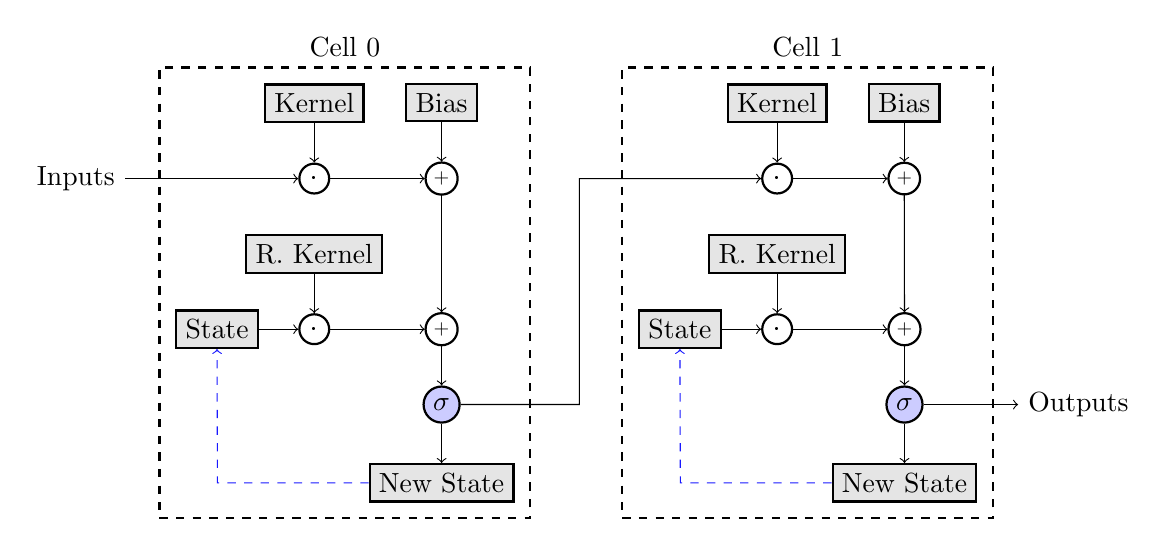
\begin{tikzpicture}[
    every node/.style={draw, thick},
    operation/.style={circle, inner sep=2pt},
    kernel/.style={rectangle, fill=gray!20},
    point/.style={coordinate},
    cell/.style={rectangle, draw, thick, dashed, inner sep=2mm, fit=#1}
]

% Cell 0
\node[kernel] (c0_kernel) {Kernel};
\node[operation, below=5mm of c0_kernel] (c0_dot1) {·};
\node[operation, right=12mm of c0_dot1, scale=0.73] (c0_add1) {+};
\node[kernel, above=5mm of c0_add1] (c0_bias) {Bias};
\node[kernel, below=5mm of c0_dot1] (c0_recur_kernel) {R. Kernel};
\node[operation, below=5mm of c0_recur_kernel] (c0_dot2) {·};
\node[kernel, left=5mm of c0_dot2] (c0_state) {State};
\node[operation, right=12mm of c0_dot2, scale=0.73] (c0_add2) {+};
\node[operation, below=5mm of c0_add2, fill=blue!20] (c0_activation) {$\sigma$};
\node[kernel, below=5mm of c0_activation] (c0_new_state) {New State};

\draw[->] (c0_kernel) -- (c0_dot1);
\draw[->] (c0_dot1) -- (c0_add1);
\draw[->] (c0_bias) -- (c0_add1);
\draw[->] (c0_add1) -- (c0_add2);
\draw[->] (c0_recur_kernel) -- (c0_dot2);
\draw[->] (c0_state) -- (c0_dot2);
\draw[->] (c0_dot2) -- (c0_add2);
\draw[->] (c0_add2) -- (c0_activation);
\draw[->] (c0_activation) -- (c0_new_state);

% Cell 1
\node[kernel, right=4.6cm of c0_kernel] (c1_kernel) {Kernel};
\node[operation, below=5mm of c1_kernel] (c1_dot1) {·};
\node[operation, right=12mm of c1_dot1, scale=0.72] (c1_add1) {+};
\node[kernel, above=5mm of c1_add1] (c1_bias) {Bias};
\node[kernel, below=5mm of c1_dot1] (c1_recur_kernel) {R. Kernel};
\node[operation, below=5mm of c1_recur_kernel] (c1_dot2) {·};
\node[kernel, left=5mm of c1_dot2] (c1_state) {State};
\node[operation, right=12mm of c1_dot2, scale=0.73] (c1_add2) {+};
\node[operation, below=5mm of c1_add2, fill=blue!20] (c1_activation) {$\sigma$};
\node[kernel, below=5mm of c1_activation] (c1_new_state) {New State};

\draw[->] (c1_kernel) -- (c1_dot1);
\draw[->] (c1_dot1) -- (c1_add1);
\draw[->] (c1_bias) -- (c1_add1);
\draw[->] (c1_add1) -- (c1_add2);
\draw[->] (c1_recur_kernel) -- (c1_dot2);
\draw[->] (c1_state) -- (c1_dot2);
\draw[->] (c1_dot2) -- (c1_add2);
\draw[->] (c1_add2) -- (c1_activation);
\draw[->] (c1_activation) -- (c1_new_state);

% Enclose cells
\node[cell=(c0_kernel)(c0_activation)(c0_state)(c0_new_state), label=above:Cell 0] {};
\node[cell=(c1_kernel)(c1_activation)(c1_state)(c1_new_state), label=above:Cell 1] {};

% Inputs and outputs
\node[rectangle, left=22mm of c0_dot1, draw=none] (input) {Inputs};
\node[rectangle, right=1.2cm of c1_activation, draw=none] (output) {Outputs};

\draw[->] (input) -- (c0_dot1);

% Modified arrows
\draw[->] (c0_activation) -- ++(1.75,0) -- ++(0,2.87) -- (c1_dot1.west);
\draw[->, dashed, draw=blue!90] (c0_new_state.west) -- ++(-1.92,0) -- (c0_state.south);
\draw[->, dashed, draw=blue!90] (c1_new_state.west) -- ++(-1.92,0) -- (c1_state.south);

\draw[->] (c1_activation) -- (output);

\end{tikzpicture}
\end{document}
